\documentclass{jsarticle}
\usepackage[dvipdfmx]{graphicx}
\usepackage{bm}
\usepackage{amsmath}
\usepackage{amssymb}
\usepackage{amsfonts}
\usepackage{comment}
\usepackage{listings}
\usepackage{cases}
\lstset{
    basicstyle={\ttfamily},
    identifierstyle={\small},
    commentstyle={\smallitshape},
    keywordstyle={\small\bfseries},
    ndkeywordstyle={\small},
    stringstyle={\small\ttfamily},
    frame={tb},
    breaklines=true,
    columns=[l]{fullflexible},
    numbers=left,
    xrightmargin=0zw,
    xleftmargin=3zw,
    numberstyle={\scriptsize},
    stepnumber=1,
    numbersep=1zw,
    lineskip=-0.5ex,
    keepspaces=true,
    language=c
}
\renewcommand{\lstlistingname}{リスト}
\makeatletter
\newcommand{\figcaption}[1]{\def\@captype{figure}\caption{#1}}
\newcommand{\tblcaption}[1]{\def\@captype{table}\caption{#1}}
\makeatother

\title{科学技術英語 英文読解課題}
\author{Ec5 24番 平田 蓮}
\date{}

\begin{document}
\maketitle
\section*{付録A 発展的なNumPy}
    この付録では、配列計算のためのNumPyライブラリをより深く掘り下げていきます。
    これにはndarray型の内部の詳細や、より高度な配列操作とそのアルゴリズムが含まれます。

    この付録は雑多な内容を含んでおり続けて読む必要はありません。

    \subsection*{A.1 ndarrayオブジェクトの内部構造}
        NumPyのndarrayは、同じ型のデータのブロックを
        (連続か区切られているかにかかわらず)
        多次元配列オブジェクトとして提供します。
        データ型(dtype)は、データが浮動小数点、整数、真偽値、
        あるいはこれまで見てきた他の型のどれであるかを決定します。

        ndarrayを柔軟にしている理由の一つに、
        すべての配列オブジェクトがデータをブロック区切りでみていることがあります。
        例えば配列に対する参照\verb|arr[::2, ::-1]|がデータを一切コピー
        していないことを不思議に思うかもしれません。
        その理由は、ndarrayは単なるデータとその型の集まりではなく、
        配列がメモリ内をさまざまなステップサイズで移動できるようにする「ストライド」
        情報を持っているからです。
        より正確に言うと、ndarrayの内部は以下のような構成になっています。

        \begin{itemize}
            \item RAMやメモリマップ内にあるデータの集まりへのポインタ
            \item 配列内の一定個数のデータの型
            \item 配列の形を表すタプル
            \item 各次元に沿って要素を一つ進めるために遷移するバイト数(整数値)のタプル
        \end{itemize}

        図\ref{fig:A-1}は、ndarrayの内部構造を示す模式図です。

        \begin{figure}[h]
            \centering
            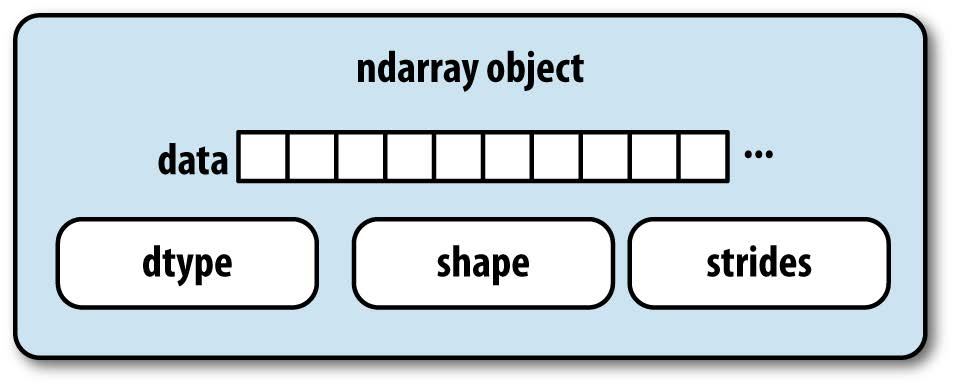
\includegraphics[width=10cm]{images/A-1.jpg}
            \caption{NumPyのndarrayオブジェクト}
            \label{fig:A-1}
        \end{figure}

        例えば、10 $\times$ 5の配列は\verb|(10, 5)|の形を持っています。

        \begin{lstlisting}
np.ones((10, 5)).shape # (10, 5)\end{lstlisting}

        float64(8バイト)型の典型的な3$\times$4$\times$5配列は、
        \verb|(160, 40, 8)|のストライドを持っています。
        (一般的に特定の軸のストライドが大きいほど、
        その軸に沿って計算を行うコストが高くなるので、
        ストライドについて知っておくと便利です。)

        \begin{lstlisting}
np.ones((3, 4, 5), dtype=np.float64).strides # (160, 40, 8)\end{lstlisting}

        典型的なNumPyユーザーが配列のストライドに興味を持つことは稀ですが、
        ストライドは0配列をコピー、構築するための重要な要素です。
        ストライドには負の値を設定することもでき、
        配列をメモリ上で逆向きに移動させることができます
        (例えば、\verb|obj[::-1]|や\verb|obj[:, ::-1]|
        のようなスライスがこれに該当します)。

        \subsubsection*{NumPyのdtypeの階層構造}
            配列の中に整数、浮動小数点数、文字列、
            Pythonオブジェクトが含まれているかどうかのチェックが
            必要なコードがあるかもしれません。
            浮動小数点数には複数の型(float16~float128)があるため、
            その配列のdtypeが型一覧の中にあるかどうかをチェックするのは非常に冗長です。
            幸い、dtypeには\verb|np.integer|や\verb|np.floating|
            などのスーパークラスがあり、
            \verb|np.issubdtype()|と組み合わせて使用することができます。

            \begin{lstlisting}
ints = np.ones(10, dtype=np.uint16)
floats = np.ones(10, dtype=np.float32)

np.issubdtype(ints.dtype, np.integer) # True
np.issubdtype(floats.dtype, np.floating) # True\end{lstlisting}

            特定のdtypeの親クラスをすべて見るには、
            その型の\verb|mro|メソッドを呼び出します。

            \begin{lstlisting}
np.float64.mro() # [numpy.float64, numpy.floating, numpy.inexact, numpy.number, numpy.generic, float, object]\end{lstlisting}

            図\ref{fig:A-2}は、dtypeの階層と親、サブクラスの関係を示したものです。

            \begin{figure}[h]
                \centering
                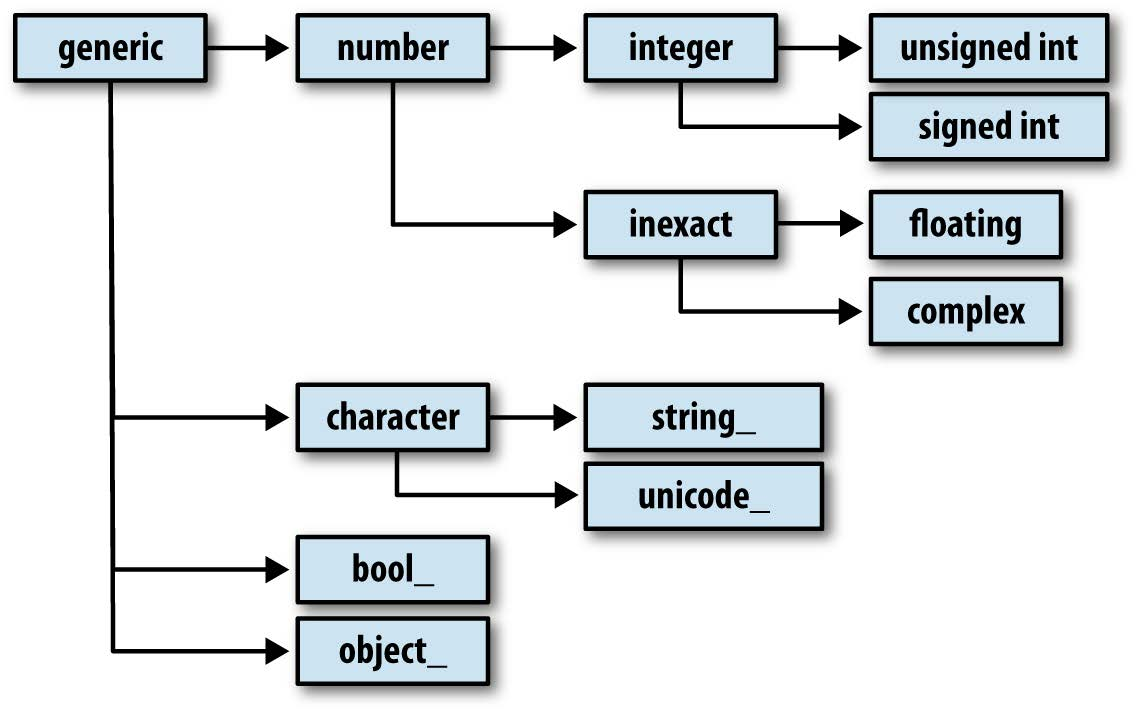
\includegraphics[width=10cm]{images/A-2.jpg}
                \caption{NumPyのdtypeの階層構造}
                \label{fig:A-2}
            \end{figure}

    \subsection*{A.2 発展的な配列操作}
        配列を扱う方法には、インデックス、スライス、ブーリアン
        のサブセットといった洒落た方法以外のものもたくさんあります。
        データ分析アプリケーションの大部分はpandasの高レベル関数で処理されますが、
        既存のライブラリにはないデータアルゴリズムを書かなければならない
        場合もあるでしょう。

        \subsubsection*{配列の変形}
            多くの場合、データを一切コピーせずに
            配列を他の形へ変形できます。
            そのためには、配列の\verb|reshape|メソッドに新しい形を表す
            タプルを渡します。
            例えば、ある値を持つ一次元の配列を行列に並べ替えたいとします。
            (結果は図\ref{fig:A-3}の通りです。)

            \begin{lstlisting}
arr = np.arange(8) # [0, 1, 2, 3, 4, 5, 6, 7]
arr.reshape((4, 2)) # [[0, 1], [2, 3], [4, 5], [6, 7]]\end{lstlisting}

            \begin{figure}[h]
                \centering
                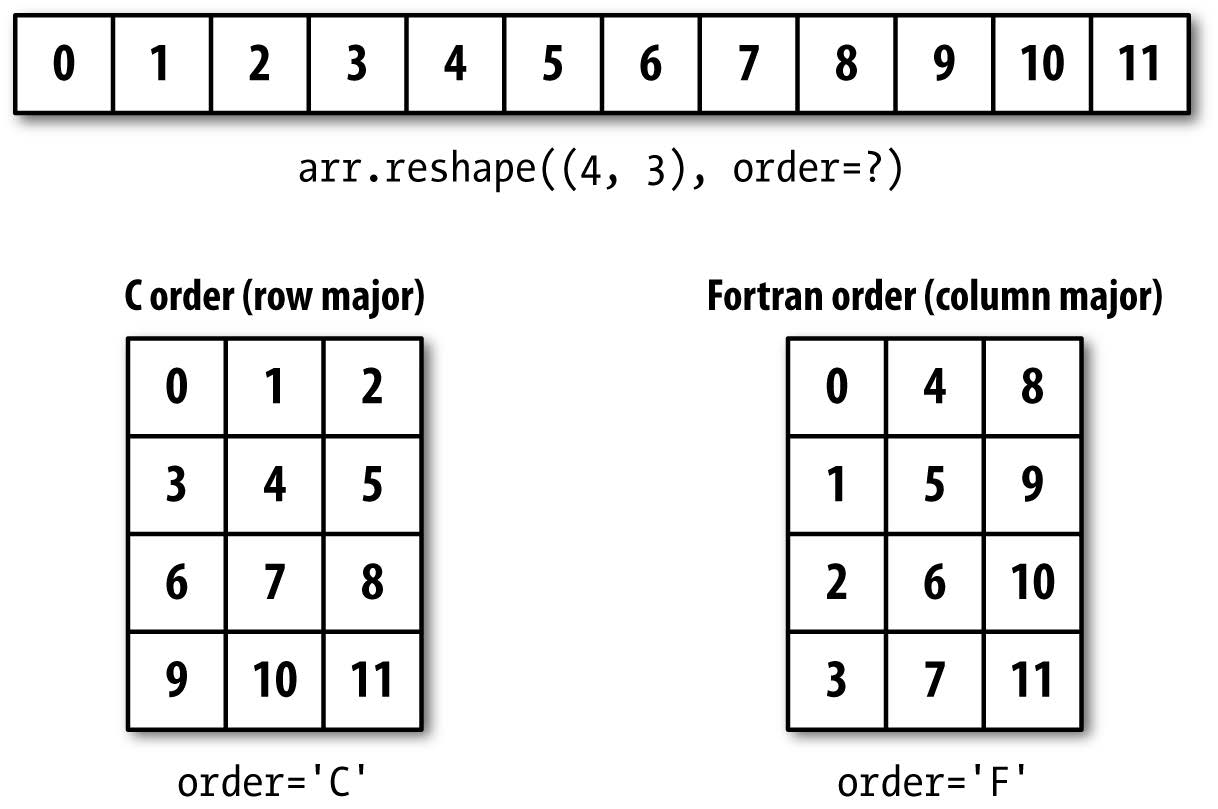
\includegraphics[width=10cm]{images/A-3.jpg}
                \caption{C(行優先)順序とFortran(列優先)順序での変形}
                \label{fig:A-3}
            \end{figure}

            多次元配列は次のように変形することもできます。

            \begin{lstlisting}
arr.reshape((4, 2)).reshape((2, 4)) # [[0, 1, 2, 3], [4, 5, 6, 7]]\end{lstlisting}

            形を表す次元数のうち、一つは-1にすることが可能で、
            その場合、その次数はデータから推測されます。

            \begin{lstlisting}
arr = np.arange(15)
arr.reshape((5, -1)) # [[ 0, 1, 2], [ 3, 4, 5], [ 6, 7, 8], [ 9, 10, 11], [12, 13, 14]]\end{lstlisting}

            配列の\verb|shape|属性はタプルであるので、\verb|reshape()|に渡すことも可能です。

            \begin{lstlisting}
other_arr = np.ones((3, 5))
other_arr.shape # (3, 5)
arr.reshape(other_arr.shape) # [[ 0, 1, 2, 3, 4], [ 5, 6, 7, 8, 9], [10, 11, 12, 13, 14]]\end{lstlisting}

            一次元から高次元への変形の逆の操作は一般的に
            フラットニングやラベリングと呼ばれます。

            \begin{lstlisting}
arr = np.arange(15).reshape((5, 3)) # [[ 0, 1, 2], [ 3, 4, 5], [ 6, 7, 8], [ 9, 10, 11], [12, 13, 14]]
arr.ravel() # [ 0, 1, 2, 3, 4, 5, 6, 7, 8, 9, 10, 11, 12, 13, 14]\end{lstlisting}

            \verb|ravel()|は変形後の値が隣接している場合、元の値をコピーしません。
            \verb|flatten|メソッドは常にデータのコピーを返すという点を除いて、
            \verb|ravel|と同じ動作をします。

            \begin{lstlisting}
arr.flatten() # [ 0, 1, 2, 3, 4, 5, 6, 7, 8, 9, 10, 11, 12, 13, 14]\end{lstlisting}

            データは違う順序で変形したり、ラベリングしたりすることができます。
            これは、NumPyの新規ユーザーにとっては少しニュアンスの異なるトピック
            であるため、次のサブトピックになっています。

        \subsubsection*{C順序とFortran順序}
            NumPyは、メモリ上のデータのレイアウトをコントロールし、
            柔軟に変更することができます。
            デフォルトでは、NumPyの配列は行優先に作成されます。
            これは空間的には、データの2次元配列を持っている場合、
            配列の各行のアイテムは隣接するメモリ位置に格納されることを意味します。
            歴史的な理由から、行と列の主要な順序は、
            それぞれCとFortranの順序としても知られています。
            FORTRAN 77言語では、行列はすべて列優先の順序で表されます。
            これは通常、「C」または「F」のように設定できます
            (他にもよく使われるオプション「A」と「K」があります)。

        \subsubsection*{配列の結合・分割}
            \verb|np.concatenate|は、配列を受け取り、
            入力の軸に従って結合します。

            \begin{lstlisting}
arr1 = np.array([[1, 2, 3], [4, 5, 6]])
arr2 = np.array([[7, 8, 9], [10, 11, 12]])

np.concatenate([arr1, arr2], axis=0) # [[ 1,  2,  3],[ 4,  5,  6],[ 7,  8,  9],[10, 11, 12]]
np.concatenate([arr1, arr2], axis=1) # [[ 1,  2,  3,  7,  8,  9],[ 4,  5,  6, 10, 11, 12]]\end{lstlisting}

            \verb|vstack|や\verb|hstack|などの
            便利な関数があります。
            これらは次のような働きをします。

            \begin{lstlisting}
np.vstack((arr1, arr2)) # [[ 1,  2,  3],[ 4,  5,  6],[ 7,  8,  9],[10, 11, 12]]
np.hstack((arr1, arr2)) # [[ 1,  2,  3,  7,  8,  9],[ 4,  5,  6, 10, 11, 12]]\end{lstlisting}

            \verb|split|は逆に、配列を入力の軸に従って分割します。

            \begin{lstlisting}
arr = np.random.randn(5, 2) # [[-0.2047,  0.4789],[-0.5194, -0.5557],[ 1.9658,  1.3934],[ 0.0929,  0.2817],[ 0.769 ,  1.2464]]
np.split(arr, [1, 3]) # [[-0.2047,  0.4789]], [[-0.5194, -0.5557],[ 1.9658,  1.3934]], [[ 0.0929,  0.2817],[ 0.769 ,  1.2464]]\end{lstlisting}

            引数の\verb|[1, 3]|は、配列を分割する添字を示しています。

            関連するすべての連結・分割関数の一覧は表\ref{tab:consp}を参照してください。
            中には非常に汎用性の高い\verb|concatenate|
            の利便性のためだけに提供されているものもあります。

            \begin{table}[h]
                \centering
                \caption{配列を連結・分割する関数}
                \label{tab:consp}
                \begin{tabular}{l|l}
                    関数 & 説明 \\ \hline
                    \verb|concatenate| & 一般的な関数。一方向に複数の配列を結合する。\\
                    \verb|vstack|, \verb|row_stack| & 行方向に配列を結合する。\\
                    \verb|hstack| & 列方向に配列を結合する。\\
                    \verb|column_stack| & \verb|hstack|と同じだが、最初に一次元配列を二次元列ベクトルに変換する。\\
                    \verb|dstack| & 奥行き方向に配列を結合する。\\
                    \verb|split| & 特定の軸方向に、指定した添字で配列を分割する。\\
                    \verb|hsplit|, \verb|vsplit| & それぞれ\verb|split|を行方向、列方向に行う。
                \end{tabular}
            \end{table}

        \subsubsection*{おしゃれな配列参照}
            整数の配列を用いて、少し変わった参照を行うことができます。

            \begin{lstlisting}
arr = np.arange(10) * 100 # [0, 100, 200, 300, 400, 500, 600, 700, 800, 900]
inds = [7, 1, 2, 6]

arr[inds] # [700, 100, 200, 600]\end{lstlisting}

            似た働きをする関数、\verb|take|と\verb|put|があります。

            \begin{lstlisting}
arr.take(inds) # [700, 100, 200, 600]
arr.put(inds, 42) # [0, 42, 42, 300, 400, 500, 42, 42, 800, 900]\end{lstlisting}

            \verb|put|は軸の引数を受け取らず,
            C順に一次元化された配列にインデックスを付けます。
            このように、他の添字配列を使用して要素を設定する必要
            がある場合は多くの場合、この参照方法を使用するのが最も簡単です。
    \subsection*{A.3 ブロードキャスト}
        ブロードキャストは、
        異なる形状の配列間での演算方法を表現したものです。
        これは強力な機能ですが、経験豊富なユーザでも混乱することがあります。
        最も簡単なブロードキャストの例は、
        スカラ値と配列の組み合わせです。

        \begin{lstlisting}
r = np.arange(5) # array([0, 1, 2, 3, 4])
arr * 4 # array([ 0,  4,  8, 12, 16])\end{lstlisting}

        これは、スカラー値である4が乗算の際に他のすべての要素に
        ブロードキャストされたことを示しています。
        例えば、配列の各列の平均値を減算することで、
        列を小さくすることができます。これは、非常に簡単です。

        \begin{lstlisting}
r = np.random.randn(4, 3)
arr.mean(0) # array([-0.3928, -0.3824, -0.8768])
demeaned = arr - arr.mean(0) # array([[ 0.3937,  1.7263,  0.1633],[-0.4384, -1.9878, -0.9839],[-0.468 ,  0.9426, -0.3891],[ 0.5126, -0.6811,  1.2097]])
demeaned.mean(0) # array([-0.,  0., -0.])\end{lstlisting}

    \subsection*{A.4 発展的なufuncの使い方}
        多くのNumPyユーザーは、
        ユニバーサル関数が提供する高速な要素間演算のみを利用するでしょうが、
        ループなしでより簡潔なコードを書くのに役立つ追加機能がいくつかあります。

        \subsubsection*{ufuncインスタンスメソッド}
            NumPyのバイナリ関数には、
            ある種の特殊なベクトル演算を行うための特別なメソッドがあります。
            \verb|reduce|は、1つの配列を受け取り、
            一連のバイナリ操作を実行することで、その値を集約します。
            例えば、配列の要素の合計を求めるには、
            \verb|np.add.reduce|を使用します。

            \begin{lstlisting}
arr = np.arange(10)
np.add.reduce(arr) # 45
arr.sum() # 45  
\end{lstlisting}

            開始値(addの場合は0)はufuncに依存します。
            軸が渡された場合、その軸に沿って演算が実行されます。
            これにより、ある種の値を簡潔に答えることができます。
            具体的な例としては、\verb|np.logical_and|を使って
            配列の各行の値がソートされているかどうかを調べることができます。
            (ここで、\verb|logical_and.reduce|と\verb|all|は同じ働きをします。)

            \begin{lstlisting}
np.random.seed(12346)
arr = np.random.randn(5, 5)
arr[::2].sort(1)
arr[:, :-1] < arr[:, 1:] # array([[ True,  True,  True,  True],[False,  True, False, False],[ True,  True,  True,  True],[ True, False,  True,  True],[ True,  True,  True,  True]], dtype=bool)

np.logical_and.reduce(arr[:, :-1] < arr[:, 1:], axis=1) # array([ True, False,  True, False,  True], dtype=bool)\end{lstlisting}

    \subsection*{A.5 構造化配列と記憶配列}
        これまで、ndarrayは同種のデータコンテナであるように触れてきました。
        つまり、各要素がdtypeによって決められた同じバイト数を占めるメモリブロックを表しています。
        これでは一見、異質なデータや表形式のデータを表現できないように見えます。
        構造化配列とは、各要素がC言語の構造体(「構造化」という名前の由来)や、
        複数の名前付きフィールドを持つSQLテーブルの行に相当すると考えられる配列です。

        構造化されたデータタイプを指定するにはいくつかの方法があります
        (オンラインのNumPyドキュメントを参照してください)。
        典型的な方法の1つは、
        \verb|(field_name, field_data_type)|のタプルのリストとして指定する方法です。
        この場合、配列の要素はタプルのようなオブジェクトで、
        その要素は辞書型のようにアクセスできます。

        フィールド名は、dtype.names属性に格納されています。
        構造化配列のフィールドにアクセスすると、
        データのストライドビューが返されるため、何もコピーされません。
        \subsubsection*{なぜ構造化配列を使うのか}
            NumPyの構造化配列は、pandasのDataFrameなどと比較して、
            比較的低レベルなツールです。
            構造化配列は、メモリブロックを任意の複雑な入れ子構造の列を持つ表形式の構造として
            解釈する手段を提供します。
            構造化配列の各要素は、メモリ上では固定のバイト数で表現されるため、
            構造化配列のもう一つの一般的な用途として、
            固定長レコードのバイトストリームとしてデータファイルを記述することがありますが、
            これはCやC++コードでデータを並べる一般的な方法であり、
            産業界のレガシーシステムでしか見られません。
            ファイルのフォーマット(各レコードのサイズ、各要素の順序、バイトサイズ、データタイプ)がわかっていれば、
            \verb|np.fromfile|でデータをメモリに読み込むことができます。
            このような特殊な使い方は本書では説明できませんが、
            このようなことが可能であることを知っておくとよいでしょう。
\end{document}